% ====================================================================
%+
% SECTION:
%    AGN_Census.tex
%
% CHAPTER:
%    agn.tex
%
% ELEVATOR PITCH:
%-
% ====================================================================

% \section{AGN Selection and Census}
\section{AGN Selection and Census}\label{sec:AGNCensus}
\def\secname{\chpname:census}\label{sec:\secname}

\credit{ohadshemmer},
\credit{nielbrandt},
\credit{GordonRichards},
\credit{AstroVPK},
\credit{ScottAnderson}

The basic figure of merit for AGN science is the total number of AGNs
discovered in the entire LSST survey, as a function of luminosity and
redshift. The main goal is therefore to adjust the Observing Strategy
in order to maximize this number.
%The primary goal for AGN science is to maximize the discovery of AGN
%with the LSST and construct the largest possible inventory of sources
%spanning the widest possible ranges in the redshift-luminosity parameter
%space. This, in turn, will provide 
Doing so will provide tighter constraints within the context
of various cosmological science cases, such as quasar clustering,
$z>6$ quasars and reionization, and strong gravitational lensing.

% --------------------------------------------------------------------

% \subsection{Target measurements and discoveries}
\subsection{Target measurements and discoveries}
\label{sec:\secname:targets}

It is expected that $\approx 10^7 - 10^8$ AGNs will be selected in the
main LSST survey using a combination of criteria, split broadly into
four categories: colors, astrometry, variability, and multiwavelength
matching with other surveys \citep{2009arXiv0912.0201L, 2013AAS...22124710S}.
The LSST Observing strategy will mostly affect the first three of these
categories as described further below.

{\bf Colors:} The LSST observing strategy will determine the depth in each band,
as a function of position on the sky, and will thus affect the color selection
of AGNs. Additionally, it will affect the reliability of the actual
determination of the color, due to the non-negligible time gaps between
observations using two different filters for a particular LSST field. This will
eventually determine the AGN $L-z$ distribution and, in particular, may affect
the identification of quasars at $z\gtsim 6$ if, for example, $Y$-band exposures
will not be sufficiently deep.

{\bf Variability:} AGNs can be effectively distinguished from (variable)
stars, and from quiescent galaxies, by exhibiting certain characteristic
variability patterns (e.g., \citealt{ButlerandBloom2011}). Picking the
right cadence can increase the effectiveness of AGN selection. Ultimately,
hybrid color and variability algorithms will be employed to enhance
the selection process (e.g., \citealt{Petersetal2015}); this may be
particularly important for selecting obscured sources which comprise a
significant fraction of the entire AGN population.

%Non-uniform
%sampling may ``contaminate'' the variability signal of AGN candidates.

{\bf Astrometry:} In cases where selection by color and variability is
insufficient for a reliable identification, AGNs can be further selected
among sources having zero proper motion, within the uncertainties. The
LSST cadence may affect the level of this uncertainty in each band, and
may therefore affect the ability to identify (mostly fainter) AGN.
%
Differential chromatic refraction (DCR), making use of the astrometric offset a
source with emission lines has with respect to a source with a featureless
power-law spectrum, can help in the selection of AGNs and in confirming their
photometric redshifts \citep{KaczmarczikEtal2009}. The DCR effect is more
pronounced at higher airmasses. Therefore, it could be advantageous to have at
least one visit, per source, at airmass greater than about 1.4 (though of course
there are trade-offs versus the additional extinction, for faint sources). AGN
selection and photometric redshift confirmation may be affected since the LSST
cadence will affect the airmass distribution, in each band, for each AGN
candidate.
%
The deep drilling fields (DDFs) will provide a truth table for determining
the predictive power of the DCR method as a function of the airmass
distribution of the observations.

The most critical measurement for the AGN census is having a reliable
and precise redshift for each source, obtained both from a photometric
and an `astrometric' redshift from DCR.


% --------------------------------------------------------------------

% \subsection{Metrics}
\subsection{Metrics}
\label{sec:\secname:metrics}

% Ideas for Metrics:
% detection - how many can LSST detect based on the luminosity function
% (depends on the depth in each band for single epoch and coadd)
% (how will this change with each DR)? @ohadshemmer

% classification - How many of these will we actually classify as quasars?
% non-simultaneous colors. variability of QSOs (how does depend on
% cadence/baseline/seasonal gaps?)

The following are most important for the AGN census:

1) Determine the mean (averaged across the sky) {\bf uncertainty on astrometric
redshifts derived from DCR} as a function of airmass, image quality, and
limiting magnitude. These uncertainties should be compared to the
corresponding uncertainties on the photomteric redshift.

2) Estimate the {\bf number of quasars at $z>6$ that LSST can discover}
during a single visit, as well as in the entire survey, and verify that
these numbers do not fall short of the original predictions. This
simply requires computing the maximum depth in the $Y$-band (for both 
single visits and the coadd), averaged across the sky for the nominal
OpSim, as well as assessing the ability to reject L and T dwarfs via astrometry.

3) Assess the effect of {\bf non-simultaneous colors on AGN selection.}
First, the term color should be clearly defined. Potential definitions
include the difference between the co-adds in two bands for the entire
survey (or at a certain point in time during the survey), the difference
between the mdian magnitude in each band during the survey, or the
difference between observations in two bands that are closely spaced in time.
Next, each source would be represented as an ellipse in color-color space.
The aim is to assess the sizes of the ellipses and how these sizes could be
minimized by perturbing the current cadence.

4) Asses how the sampling affects the selection of AGN by variability (e.g.,
interactions with red-noise power spectrum).

%4) Estimate the number of low-luminosity AGN (LLAGN) that can be
%identified during the entire survey.

% --------------------------------------------------------------------

% \subsection{OpSim Analysis}
\subsection{OpSim Analysis}
\label{sec:\secname:analysis}

% OpSim analysis: how good would the default observing strategy be, at
% the time of writing for this science project?

\begin{figure}
\centering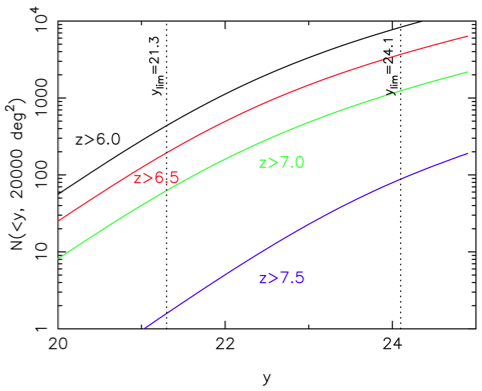
\includegraphics[width=0.9\linewidth]{figs/agn/zgt6_figure_AAS_2013.png}
\caption{Number of quasars at $z>6$ that LSST is expected to discover
based on $Y$-band limiting magnitude in a single epoch (entire survey)
marked by the first (second) dotted line from the left.}
\label{fig:zgt6}
\end{figure}


For assessing the limitations of DCR on the $L-z$ plane of LSST AGNs,
one needs to obtain from OpSim the current maximal airmasses for each band,
and the associated image quality and limiting magnitude. The current maximal
airmasses, per band, averaged across the sky are: 1.41, 1.50, 1.51, 1.51, 1.51,
and 1.51 for $u, g, r, i, z, Y$, respectively. Need to convolve this with the
seeing in each band to obtain the dependence on airmass and image
quality. This output should be converted into the mean and spread
of the uncertainty on the astrometric redshifts. The best way
to obtain this is to fold the astrometric redshift estimation from
DCR into MAF. Ultimately, one needs to check the implications of higher
airmasses and limiting magnitudes on the ability to obtain more accurate
and precise astrometric redshifts.


For predicting the number of detected $z>6$ quasars
%Compare this magnitude to the
%one required for identifying $\geq1000$ quasars at $z\geq6$.
the current 
%enigma\_1189{}
aquila\_{}1110 OpSim for the main, i.e., WFD survey, gives a
single-visit $5\sigma$-depth
%old number computed in Bremerton: $Y=22.36$ mag,
%$Y=21.51$ enigma_\_{}1189
{\it Y} $= 21.45$ mag as compared to {\it Y} $= 21.51$ for the older enigma\_{}1189 OpSim.
For the final co-added $5\sigma$-depth the median magnitude from the aquila\_{}1110
OpSim is 
%$Y=24.36$. Enigma\_{}1189
{\it Y}$ = 23.07$ which is more than a magnitude shallower than the older enigma\_{}1189 
depth of {\it Y}$ = 24.36$.
{\bf The lower {\it Y}-band depth may reduce the total number of quasars at $z > 6$ discovered by LSST by
a factor of $\sim 2$
%correspondingly deeper (i.e., better) than enigma\_{}1189
%comparable to
%the original predictions
(see Fig.~\ref{fig:zgt6}).}
% (See the AAS poster from 2013: http://www.lsst.org/sites/default/files/221-RC-247.10-AAS_shemmer.pptx.pdf).



As for general AGN selection, the effects of the sampling on variability selection
should be assessed, and the amplitudes of the uncertainties in color-color space
and how these depend on the cadence should be simulated.

% % --------------------------------------------------------------------
%
% \subsection{Discussion}
% \label{sec:\secname:discussion}
%
% Discussion: what risks have been identified? What suggestions could be
% made to improve this science project's figure of merit, and mitigate
% the identified risks?
%
%
% ====================================================================

\navigationbar
